%
% 42-methode.tex -- Die Methode
%
% (c) 2026 Prof Dr Andreas Müller
%
\subsection{Die Methode}
Die im Abschnitt~\ref{buch:integration:residuen:section:beispiel}
dargestellt Methode löst also die Aufgabe ein reelles Integral
%
% fig-methode.tex
%
% (c) 2026 Prof Dr Andreas Müller
%
\begin{figure}
\centering
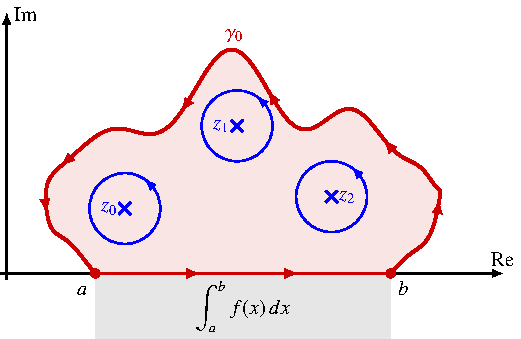
\includegraphics{chapters/030-integration/images/methode.pdf}
\caption{Die komplexe Wegintegration ermöglicht das Integral der
reellen Funktion $f(x)$ durch ein Integral einer geeigneten
komplexen Funktion $f(z)$ entlang des Weges
$\gamma_0$ und auszudrücken.
Falls im Inneren des roten Gebietes Singularitäten der Funktion $f(z)$
auftreten, symbolisiert durch die blauen Punkte, dann kommen 
noch Kurvenintegrale entlang kleinen Kreisen um die Singularitäten
hinzu.
\label{buch:integration:residuen:fig:methode}}
\end{figure}
%
\[
I
=
\int_a^b f(x)\,dx
\]
zu lösen.
Sie geht dazu wie folgt vor.

\begin{enumerate}
\item
Die reelle Funktion im Integranden muss durch eine komplexe
Funktion $f(z)$ ersetzt werden.
\item
Das Integral entlang des Segmentes $[a,b]$ auf der reellen Achse
wird durch ein Kurve $\gamma_0$ zu einem geschlossenen Weg $\gamma$
ergänzt, wie er in
Abbildung~\ref{buch:integration:residuen:fig:methode}
dargestellt ist.
\item
Falls der Integrand im Inneren der Kurve $\gamma$ holomorph ist,
verschwindet das Wegintegral.
Dann folgt, dass das Integral durch
\[
I
=
\int_a^b f(x)\,dx
=
-\int_{\gamma_0} f(z)\,dz
\]
berechnet werden kann.
\item
Falls im Inneren der Kurve $\gamma$ Singularitäten des Integranden
vorhanden sind (in der Abbildung~\ref{buch:integration:residuen:fig:methode}
durch blaue Kreuze dargestellt), muss diesen durch zusätzliche
Summanden auf der rechten Seite Rechnung getragen werden.
\index{Singularitat@Singularität}%
Da dies durch Integrale über beliebig kleine Kreise um die Singularitäten
herum geschehen kann, hängen diese Korrekturterme nur von den
Funktionswerten und Ableitungen in unmittelbarer Nähe der
Singularität ab.
Techniken zu ihrer Berechnung, insbesondere der Begriff des Residuums,
\index{Residuum}%
werden in Kapitel~\ref{chapter:analytisch} dargestellt.
Das Integral ist dann
\[
\int_a^b f(x)\,dx
=
-\int_{\gamma_0} f(z)\,dz
+
\text{Singularitätenterme.}
\]
\end{enumerate}
Da die Berechnung der Singularitätenterme, wie im einführenden Beispiel,
meist nicht schwierig ist, ist die Methode vor allem dann erfolgreich,
wenn das Wegintegral entlang $\gamma_0$ deutlich einfacher zu berechnen
ist.

Die Methode wird oft in Fällen angewendet, wo der Weg von einem
Parameter abhängt, wie im einführenden Beispiel der Radius $R$.
Wenn der gesuchte Integralwert ein Grenzwert für den Parameter ist,
kann man hoffen, dass das Integral über $\gamma_0$ im Grenzwert
deutlich einfacher zu berechnen ist.
Im Beispiel ist das Integral über den zusätzlichen Wegteil im
Grenzwert sogar verschwunden.

Im nächsten Abschnitt wird ein weiteres Beispiel für diese Methode
gezeigt. 
Ausserdem motiviert die Methode auch den Begriff des Hauptwertes,
der in Abschnitt~\ref{buch:integration:residuen:subsection:hauptwert}
skizziert und in Kapitel~\ref{chapter:hauptwert} ausführlicher
erklärt wird.
